\documentclass[border=4pt,12pt]{standalone}
% House style for redrawn exam diagrams (diagram-v4: 0.4pt lines, filled -latex arrows, fine dashes; stipple and hatching drawn as real dots/lines (no PDF/SVG patterns, so they render in every browser and at any scale); transparent background). Every figure \input's this.
\usepackage{amsmath,amssymb}
\usepackage{txfonts}
\usepackage{pdfrender,xcolor}
% \halo{text}: label on shading. The shading stops just around each letter's outline (a thin knock-out that follows the
% glyphs, like the papers' typesetting), never a box. Owner: "I don't want a box around the text".
\newcommand{\halo}[1]{\leavevmode\rlap{\pdfrender{TextRenderingMode=2,LineWidth=2.2pt,LineJoinStyle=1,StrokeColor=white,FillColor=white}#1}#1}
\usepackage{tikz,pgfplots}
\pgfplotsset{compat=1.18}
\usetikzlibrary{arrows.meta,calc,angles,quotes,patterns,patterns.meta,intersections,positioning,decorations.markings,shapes.geometric}
% Stipple and hatching are drawn as actual dots / lines clipped to the region (path picture), NOT as pattern fills:
% SVG <pattern> fills vanish or blur when browsers scale the image, so the owner could not see the shading.
% Each dot is a 0.72pt square (keeps SVGs small; reads as a dot at print size). Dots sit on one global staggered grid, so neighbouring regions line up.
\makeatletter
\newdimen\ex@x \newdimen\ex@y \newdimen\ex@xa \newdimen\ex@ya \newdimen\ex@xb \newdimen\ex@yb \newcount\ex@row
\def\exam@stipplecolor{black!75}\def\exam@dotr{0.42pt}\def\exam@dotgap{2.5}
\def\ex@rowdots{\ifdim\ex@x<\ex@xb \pgfpathrectangle{\pgfqpoint{\dimexpr\ex@x-0.36pt\relax}{\dimexpr\ex@y-0.36pt\relax}}{\pgfqpoint{0.72pt}{0.72pt}}\advance\ex@x by \exam@dotgap pt\relax\expandafter\ex@rowdots\fi}
\def\exam@stipple{%
  \pgftransformreset% dots are sized in real points even inside scaled pictures
  \pgfpointanchor{path picture bounding box}{south west}\ex@xa=\pgf@x \ex@ya=\pgf@y
  \pgfpointanchor{path picture bounding box}{north east}\ex@xb=\pgf@x \ex@yb=\pgf@y
  \pgfsetfillcolor{\exam@stipplecolor}\pgfmathsetmacro\ex@h{\exam@dotgap/2}%
  \pgfmathtruncatemacro\ex@r{floor(\ex@ya/\ex@h)-1}\ex@row=\ex@r\relax
  \ex@y=\ex@r\dimexpr\ex@h pt\relax
  \loop\ifdim\ex@y<\ex@yb
    \pgfmathtruncatemacro\ex@c{floor(\ex@xa/\exam@dotgap)-1}\ex@x=\ex@c\dimexpr\exam@dotgap pt\relax
    \ifodd\ex@row \advance\ex@x by \ex@h pt\fi
    \ex@rowdots
    \advance\ex@y by \ex@h pt \advance\ex@row by 1
    \ifnum\numexpr\ex@row-(\ex@row/4)*4\relax=0 \pgfusepath{fill}\fi% flush every 4 rows: bounded TeX memory, few clip copies in the SVG
  \repeat\pgfusepath{fill}}
\newdimen\ex@d
\def\exam@hatch#1{% #1 = 1 for /, -1 for \ ; lines 45 degrees, 3pt apart
  \pgftransformreset
  \pgfpointanchor{path picture bounding box}{south west}\ex@xa=\pgf@x \ex@ya=\pgf@y
  \pgfpointanchor{path picture bounding box}{north east}\ex@xb=\pgf@x \ex@yb=\pgf@y
  \ex@d=\dimexpr\ex@yb-\ex@ya\relax \ex@x=\dimexpr\ex@xa-\ex@d\relax
  \loop\ifdim\ex@x<\ex@xb
    \ifnum#1>0 \pgfpathmoveto{\pgfqpoint{\ex@x}{\ex@ya}}\pgfpathlineto{\pgfqpoint{\dimexpr\ex@x+\ex@d\relax}{\ex@yb}}%
    \else \pgfpathmoveto{\pgfqpoint{\ex@x}{\ex@yb}}\pgfpathlineto{\pgfqpoint{\dimexpr\ex@x+\ex@d\relax}{\ex@ya}}\fi
    \advance\ex@x by 4.24pt
  \repeat
  \pgfsetlinewidth{0.4pt}\pgfsetstrokecolor{black}\pgfusepath{stroke}}
\def\examstipple{\exam@stipple}\def\examhatch{\exam@hatch}\def\examsetstipplecolor#1{\def\exam@stipplecolor{#1}}\def\examsetdotgap#1{\def\exam@dotgap{#1}}
\makeatother
% (legacy pattern kept for old files)
% staggered stipple like the NESA papers' dotted shading
\pgfdeclarepatternformonly{exam stipple}{\pgfpointorigin}{\pgfqpoint{2.2pt}{2.2pt}}{\pgfqpoint{2.2pt}{2.2pt}}{%
  \pgfpathcircle{\pgfqpoint{0.55pt}{0.55pt}}{0.42pt}\pgfpathcircle{\pgfqpoint{1.65pt}{1.65pt}}{0.42pt}\pgfusepath{fill}}
\tikzset{
  every picture/.style={line width=0.6pt, >={Latex[length=2mm,width=1.3mm]}},
  curve/.style={line width=0.6pt},
  open arrow/.style={-{Latex[length=2mm,width=1.3mm]}},  % owner: filled -latex heads everywhere, no open chevrons
  aux/.style={dash pattern=on 2pt off 1.5pt, line width=0.6pt},
  shade/.code={\def\exA{#1}\def\exB{none}\ifx\exA\exB\else\pgfkeysalso{fill=black!18}\fi},
  shade/.default=on,
  shade dots/.style={fill=none, path picture={\examstipple}},
  stipple color/.code={\examsetstipplecolor{#1}},
  stipple gap/.code={\examsetdotgap{#1}},
  shade dense dots/.style={fill=none, stipple gap=1.6, path picture={\examstipple}},
  shade hatch/.style={fill=none, path picture={\examhatch{1}}},
  shade hatch reverse/.style={fill=none, path picture={\examhatch{-1}}},
  shade solid/.style={fill=black},
  pt/.style={circle, fill, inner sep=1.1pt},
  open pt/.style={circle, draw, fill=white, inner sep=1.1pt},
}
\pgfplotsset{
  exam axes/.style={axis lines=middle, axis line style={->}, xlabel={$x$}, ylabel={$y$},
    xlabel style={anchor=west}, ylabel style={anchor=south}, tick label style={font=\small},
    every axis plot/.append style={line width=0.6pt, black}, samples=200, clip=false,
    enlargelimits=false, axis on top},
}

\begin{document}
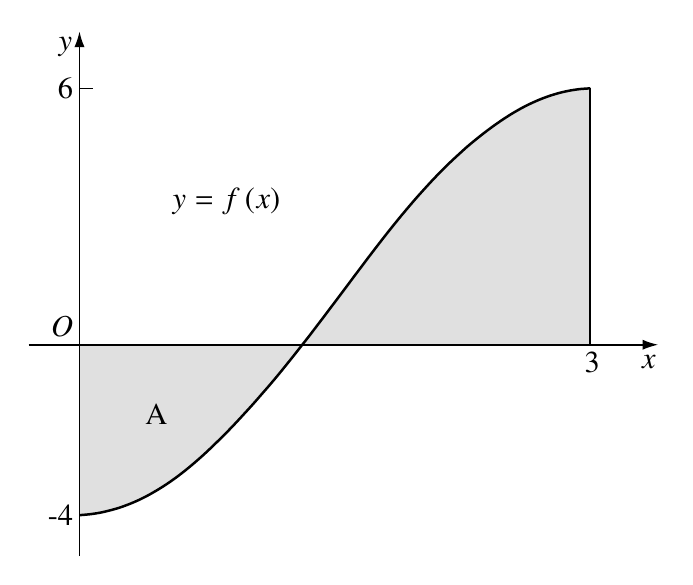
\begin{tikzpicture}[x=0.0127cm,y=-0.0127cm,font=\fontsize{11}{13}\selectfont]
  \fill[black!12] plot[smooth] coordinates {(61.0,504.0) (86.0,501.0) (110.0,493.0) (134.0,482.0) (158.0,466.0) (182.0,447.0) (206.0,424.0) (230.0,398.0) (254.0,370.0) (278.0,340.0) (283.0,333.5)} -- (61,333.5) -- cycle;
  \fill[black!12] plot[smooth] coordinates {(283,333.5) (287.4,328.1) (291.8,322.7) (296.1,317.3) (300.5,311.8) (304.8,306.4) (309.1,300.8) (313.4,295.2) (317.7,289.6) (321.9,284.1) (326.2,278.4) (330.4,272.8) (334.7,267.1) (339,261.4) (343.3,255.8) (347.6,250.1) (351.8,244.5) (356.1,239) (360.4,233.4) (364.7,227.9) (369,222.4) (373.3,216.9) (377.7,211.4) (382.1,206) (386.5,200.7) (390.9,195.4) (395.4,190.1) (399.9,184.9) (404.5,179.7) (409.1,174.6) (413.7,169.6) (418.4,164.6) (423.1,159.8) (427.9,154.9) (432.7,150.1) (437.6,145.4) (442.6,140.8) (447.6,136.3) (452.7,131.8) (457.8,127.5) (462.9,123.3) (468.1,119.3) (473.4,115.3) (478.7,111.5) (484.1,107.8) (489.6,104.3) (495.1,101) (500.7,97.87) (506.4,94.91) (512,92.19) (517.9,89.61) (523.7,87.27) (529.5,85.18) (535.5,83.27) (541.4,81.63) (547.5,80.2) (553.5,79.04) (559.6,78.12) (565.8,77.43) (572,77)} -- (572,333.5) -- cycle;
  \draw[->] (10,333.5) -- (640,333.5);
  \draw[->] (61,545) -- (61,20);
  \draw (61,77) -- (75,77);
  \node[anchor=north,inner sep=0pt] at (574,340) {$3$};
  \node[anchor=base] at (630,357) {$x$};
  \node[anchor=base] at (47,39) {$y$};
  \node[anchor=east,inner sep=2pt] at (61,77) {$6$};
  \node[anchor=east,inner sep=2pt] at (61,504) {$\text{-}4$};
  \node[anchor=base east,inner sep=2pt] at (61,325) {$O$};
  \draw[line width=0.9pt] plot[smooth] coordinates {(61,504) (71.1,503.1) (81.11,501.6) (91.2,499.3) (101,496.5) (110.6,493) (120.2,488.9) (129.7,484.1) (139.1,478.7) (148.3,472.9) (157.4,466.5) (166.4,459.6) (175.1,452.4) (184,444.6) (192.6,436.6) (201.1,428.3) (209.8,419.6) (218.2,410.8) (226.5,401.8) (234.8,392.7) (242.9,383.4) (251,374.1) (259,364.6) (266.9,354.9) (274.7,345.2) (282.4,335.4) (290.2,325.5) (297.9,315.4) (305.6,305.3) (313.2,295.2) (320.9,285) (328.6,274.7) (336.3,264.4) (343.9,254.3) (351.6,244.1) (359.2,234.2) (366.8,224.4) (374.6,214.6) (382.4,205) (390.3,195.6) (398.3,186.3) (406.3,177.4) (414.4,168.6) (422.8,159.9) (431.3,151.5) (439.9,143.5) (448.6,135.6) (457.5,128.2) (466.6,121) (475.9,114.1) (485.2,107.7) (494.5,101.8) (504,96.4) (513.6,91.62) (523.1,87.51) (532.7,84.05) (542.5,81.2) (552.3,79.09) (562.1,77.69) (572,77)};
  \draw (572,77) -- (572,333.5);
  \node at (208,190) {$y=f\,(x)$};
  \node at (138,403) {A};
\end{tikzpicture}
\end{document}
